\begin{figure}[p]
\centering
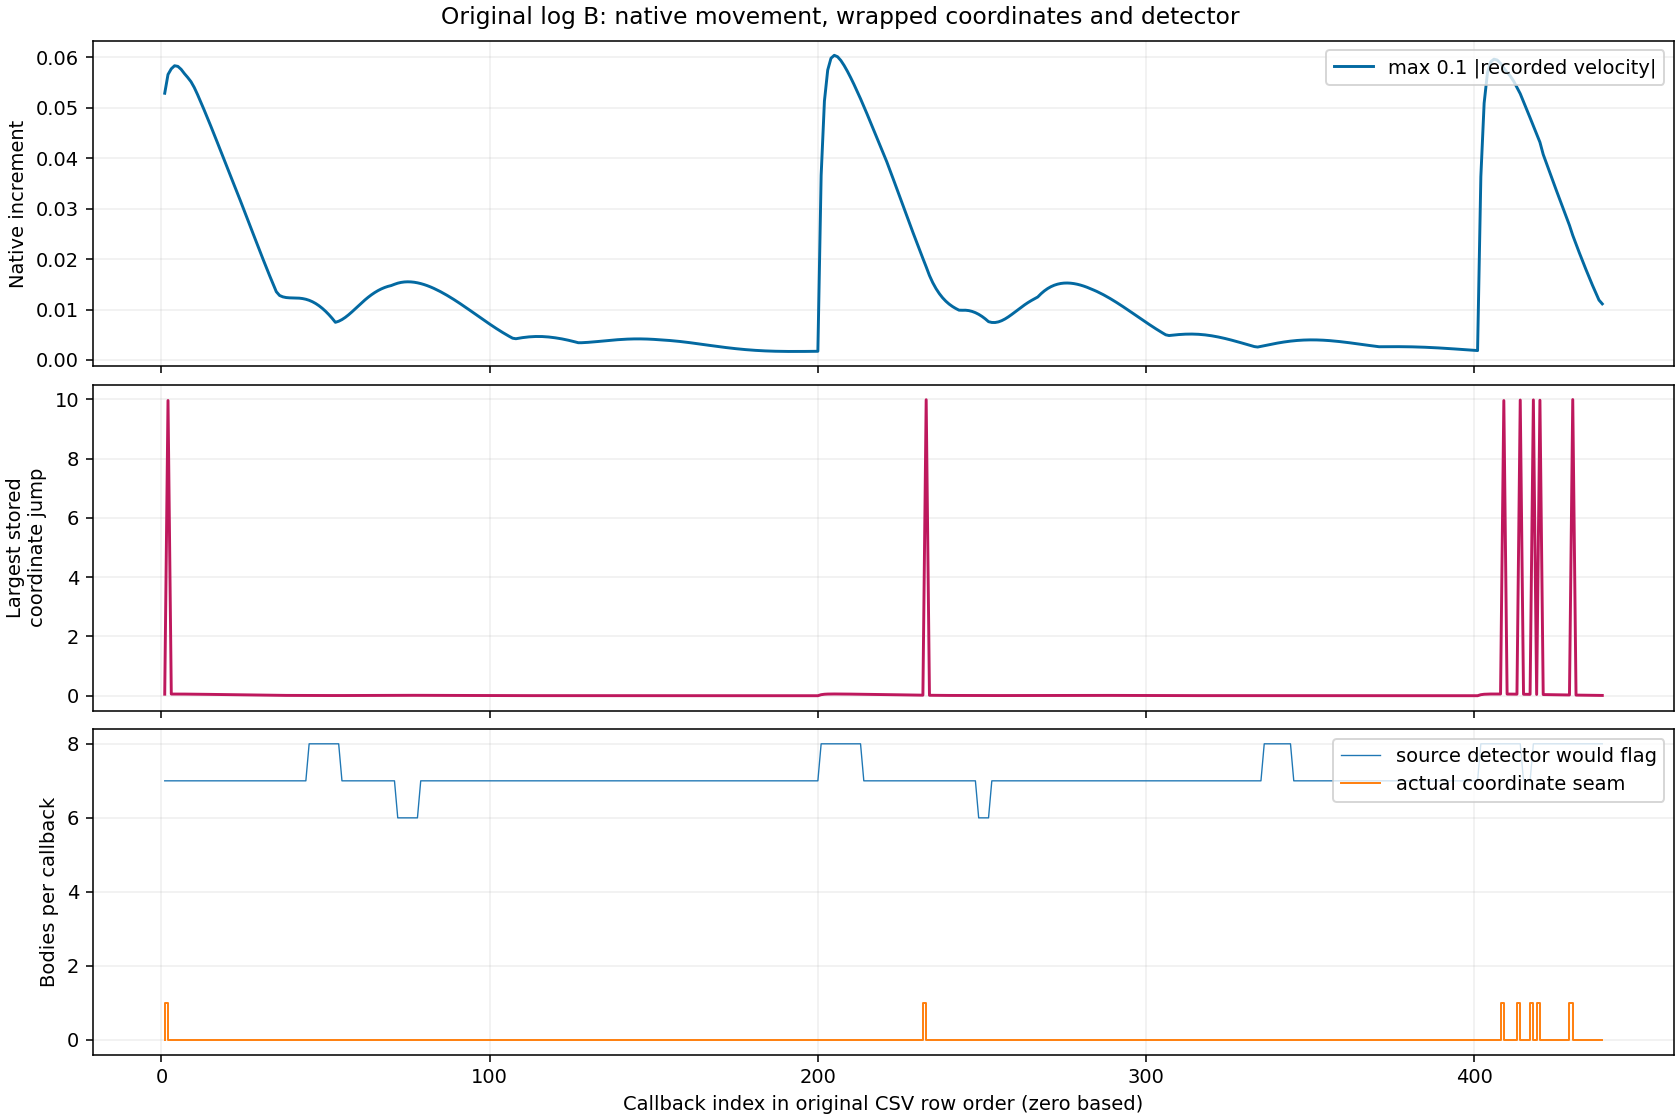
\includegraphics[width=\linewidth,height=0.70\textheight,keepaspectratio]{figures/F12_0.png}
\caption[Native increments and detector flags in log B]{DERIVED from ORIGINAL log B, reused from Study 03. Callback order preserves repeated labels. Seven actual seam body events coexist with 3129 detector would-flags; small negative coordinate differences trigger the unsigned-modulo defect. Largest checked native increment is 0.060380826 at q205/body 5. The figure does not equate a near-ten coordinate jump with travel of that length. \cite{study03}}
\label{fig:F12}
\end{figure}
